\chapter{Related Work}
\label{ch:related}


%In this chapter, we focus on previous work that is related to the problem stated in \nameref{ch:introduction}. 
This section reviews the state-of-art of research works in the field of RDF syntax parsing and checking.

\section{RDF Parsing and Syntax Checking Approaches}
In order to validate RDF data as an input, either by inserting a URL where it exists or by uploading a file, almost the available tools and applications that we could find, can only offer the first detected syntax error while consecutively parsing that input from its start point to its end point. Moreover, semantic developers and engineers are struggling whilst debugging their RDF data and they necessarily need alternative tools that could be more helpful. To the best of our knowledge, there is no comparable prior work regarding fault-tolerant parsing and syntax checking of the diverse RDF serialization formats expect one that can only work for an RDF/XML format. Hence, a tool that can prominently list of all errors included in the RDF data is desired.
\subsection{RDF/XML Parsing Tools}

 Despite the existence of  several theoretical models and practical tools that have been invented in the same field, we can hardly find a research that cares of finding more than one syntax error inside RDF data. Moreover, during our journey of searching the existing tools that provide such a service, the W3C RDF validation tool \cite{W3C:Validation:Online} was firstly checked, it is an web tool, available online for the purpose of parsing and validating RDF/XML codes. It uses the ARP parser of Jena \cite{McBride:2002:JSW:613357.613755} as its core, however, it fails in detection of multiple syntax errors and the first error in order was only released as shown by Figure \ref{Fig:errorW3RDFValidator}.
 
 In 2000, a Validating RDF Parser (VRP) \cite{karsten:Thesis:2000} was developed by K. Tolle in his thesis, it is a Java-base parsing tool, features semantically and syntactically checking of an RDF/XML format. Nevertheless, the validation service provided by VRP is limited to parse only a format type of RDF/XML and does not support other RDF serialization formats, such as N3, N-Triple, and Turtle. Figure \ref{Fig:VRPErrorResult} shows that VRP can list more than one error or first detected error. An RDF/XML file with the same text applied in Figure \ref{Fig:errorW3RDFValidator}, included 2 syntax errors was used as an input to test VRP. As a result, 4 error messages were given, 2 of them are very related to the injected errors and significantly meaningful to correct them, whereas the other 2 messages are with no benefits and have no relation to them, they are false positives. Differently, in this work, a general approach that can work for all RDF serialization formats is planned, however as use cases, Turtle and N-Triple formats have been considered  while developing RDF-Doctor to prove our assumption. 
 
 \begin{figure}[ht]
		\begin{center}
			\setlength\belowcaptionskip{-7mm}
			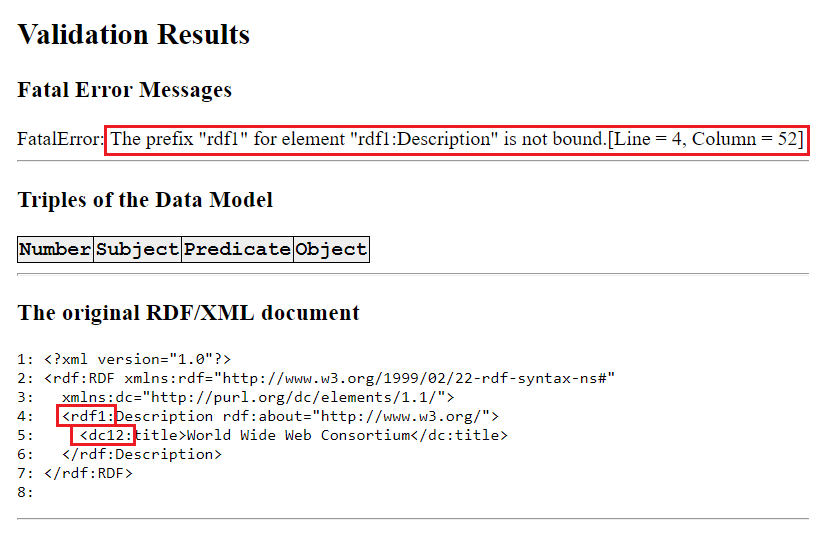
\includegraphics[scale=0.8,angle=0]{images/errorW3RDFValidator.png}
			\caption{\textbf{Validation results of the W3C RDF validation tool \cite{W3C:Validation:Online} after parsing an RDF/XML text, included two syntax errors.} the original RDF/XML document has two syntax errors since "rdf1" and "dc12" have no prefix declarations, but the results under "Fatal Error Messages"  show only the first found error and neglects the other.}
			\label{Fig:errorW3RDFValidator}
		\end{center}
	\end{figure}
\subsection{Several Serialization Formats  Parsing Tools}

\par Next, the existing tools that validate more than one  RDF serialization formats rather than only parsing of RDF/XML format were checked. We have started with Jena RDF toolkit \cite{McBride:2002:JSW:613357.613755} which offers validation service based on the ARP parser. It can  be also used as a standalone program using a command-line  or as an API, integrated within another application. Considering its powerful capability of validating numerous RDF serialization formats, including RDF/XML, again, the first error is only reported.
 \begin{figure}[ht]
		\begin{center}
			\setlength\belowcaptionskip{-10mm}
			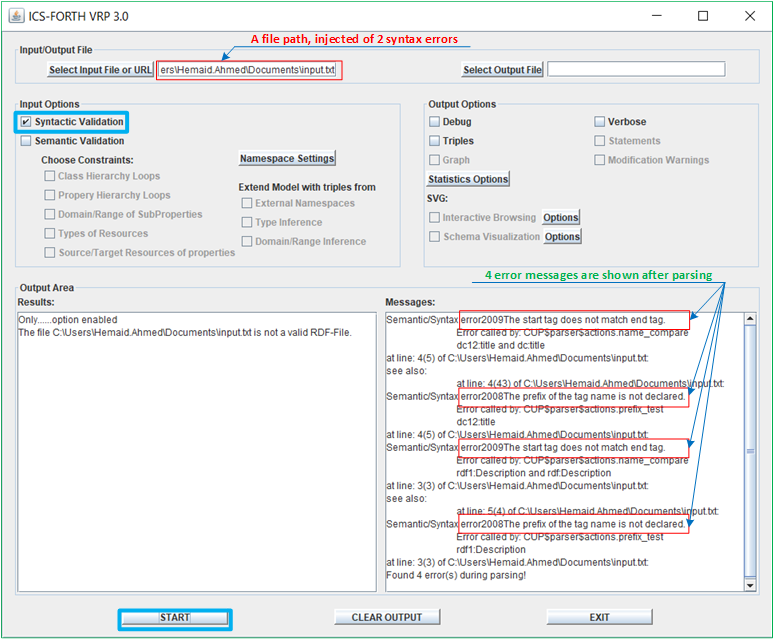
\includegraphics[scale=0.7,angle=0]{images/VRPErrorResult.png}
			\caption{\textbf{Validation results of Validating RDF Parser (VRP) \cite{karsten:Thesis:2000} after parsing an RDF/XML file, included two syntax errors.} 4 error messages are shown, 2 of them are meaningful, hence, they help in resolving the 2 detected errors, the other 2 messages have no meaning}
			\label{Fig:VRPErrorResult}
		\end{center}
	\end{figure}
\subsection{Classification of parsing approaches based on its core}

Some of the tools validating RDF formats use the following core tools or methods as a significant part of their implementations. which tool  uses which core component is discussed in the following : \begin{itemize}[noitemsep] 
	\item \textbf{ARP-parser-dependable approach :} both W3C RDF validation tool \cite{W3C:Validation:Online} and RDF Validator and Converter \cite{Mybluemix:Validation:Online} use the ARP parser of Jena framework \cite{McBride:2002:JSW:613357.613755}. However, the latter focuses more on triple-based serialization formats, validating them and converting from one format to another, whereas the former validates only RDF/XML format. 
	\item \textbf{N3-parser-dependable approach :} N3 parser \cite{N3Parser:Online} is a JavaScript\_based syntax validator, mainly, developed for checking the syntax of Turtle and N-Triple formats. The online version of IDLab Turtle Validator \cite{IDLab:Validation:Online} uses N3 parser and it is integrated as a NodeJS plug-in. As well, the same approach was used to build a turtle editor with syntax validation in \cite{petersenturtleeditor}. However, this approach is slow when parsing and its behaviour is unpredictable when dealing with large files. 
	\item \textbf{Shape expressions approach:} in \cite{prud2014shape} a turtle parser was developed based on shape expressions. Shape expressions validates RDF through declaring of constraints on the RDF data, if the declared constraints are violated, then RDF data is invalid, otherwise, it is valid. Furthermore, Shape expressions describes the RDF graph based on regular expressions. 
\end{itemize} 

The previous three approaches failed to list more than the first found error. Another essential point has been learned is to avoid JavaScript\_based development of the new tool and the alternative is to use Java\_based application, similar to the ARP-parser discussed in the first approach. Empirically, developing using java can improve the performance of the purposed tool, especially when  validating large RDF data files.

\section{Types of Error Messages Approaches}
Releasing user-friendly and meaningful error messages is of a great benefit to help the user to identify and correct the errors. 
\begin{itemize}
    \item \textbf{Non-expressive and meaningless error messages:} the parsing tools under the Shape expressions approach show less expressive  and unfriendly error messages.
    \item \textbf{Expressive error and meaningful  messages:} the parsing tools of ARP-parser-dependable approach and N3-parser-dependable approach  are presenting more expressive and user-friendly error messages which can provide the syntax error and its location in a proper way. 
    
\end{itemize}

\section{Error Recovery Approach}
Automatic error recovery or correction will be valuable to resolve from common syntax errors. For example, lots of programming languages need a semicolon at the end of the line. There are also few tools which can correct such errors without the involvement of the programmer. In the same way it will be useful to have this option of automatic correction after parsing of various serialization formats of RDF. Further, while surveying the existing RDF parsing tools, a tool proposed or provided such a feature was not found. RDF-Doctor will be equipped with this feature to correct these errors.   

\par
To end this chapter, after describing the actual issue, reviewing the  state-of-art of research works, related to the same spot with pointing out  the different approaches of RDF parsing and syntax checking, different types of error messages , and finally the approach of automatic error correction. The outcome of this study is the RDF-Doctor. It is a parser that is generated with the help of the ANTLR parser generator. Additionally, It is a Java\_based application to parse N-Triple and Turtle serialization formats; show a meaningful error messages; as well as, automatically recover from common syntax errors.    










